
\chapter{FPGA, microprocesadores Soft-Core y System on Chip}
	

\section{FPGAs}

	\subsection{Introducción}
La fabricación de dispositivos semiconductores es un proceso complicado de plazos largos y costoso. Esto lleva a que los diseños destinados para la  implementacion en chip de silicio tengan poco oportunidad de ser prototipados antes de que comience la producción en grandes volúmenes. Esto supone una gran importancia  en las faces de prueba y verificación de un diseño antes de ser fabricado.

Basándose en la predicción de la ley de Moore donde expresa que aproximadamente cada dos años se duplica el número de transistores en un circuito integrado\cite{Etiqueta02}, Ross Freeman postulo que los transistores serian menos costoso cada año, haciendo asequible la fabricación de chips programables personalizables \cite{Etiqueta03}.
La compañía Xilinx, ofreció su primer chip en 1984 , que contiene arrays celdas lógicas (LCAs) , programables por el usuario en casi cualquier configuración que quisieran. Estos se conocen como Field Programmable Gate Array (\textit{FPGAs}) .

Las \textit{FPGAs} desempeñan un papel dual, uno como objetivo final de ejecución en un diseño y otro papel como prototipo para la implmentacion definitiva de un diseño. Su capacidad de reconfigurar el diseño parcial o totalmente para su actualización o corrección de errores tiene un costo relativamente bajo a diferencia del prototipado sobre ASICs.
Actualmente las \textit{FPGA} cuentan con una gran cantidad de recursos disponibles (Compuertas lógicas , Bloques de RAM) para implementar diseños digitales complejos.

Una desventaja de las \textit{FPGA}  es debido a la naturaleza inherente de las arquitecturas de \textit{FPGA}, los diseños implementados en \textit{FPGA} comparados con una ASICs en general tienen mas area, menos porformance y consumen mas energía.
		
A medida que fue pasando el tiempo las FPGAs fueron disminuyendo su costo y mejoraron la eficiencia en el consumo de energía llevandolas a ser consideradas como solución a la implementacion de ciertas aplicaciones en lugar de una ASIC. Si los criterios tales como el tiempo de comercialización y capacidad de actualización son críticos, con el máximo rendimiento y un consumo reducido de energía, una implementación en  FPGA puede ser adecuada.

	\subsection{Arquitecura}
Los componentes de una \textit{FPGA} se pueden dividir en cinco grupos:

\begin {itemize}
\item  Bloques lógicos configurables y \textit{Lookup Tables}.
\item  Bloques de entrada y salida.
\item  Bloques multiplicadores
\item  Bloques Manejadores de Clock Digitales.
 \end {itemize}

\begin{figure}[h!]
 \begin{center}
   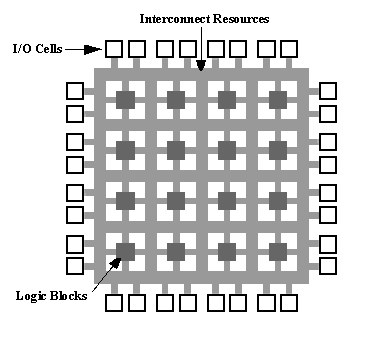
\includegraphics[width=0.5\textwidth,keepaspectratio=true]{./images/fpga1a}
  \caption{Componentes de una FPGA}
  \label{fig:esquema}
 \end{center}
\end{figure}

		\subsubsection{Bloques Lógicos Configurables y Lookup Tables}

Todas las\textit{FPGAs} se basan en arrays de pequeños elementos de lógica digital. Los problemas de lógica digital se descomponen en circuitos lógicos que puedan ser mapeados a uno o más de estas “celdas lógicas” a través de un proceso llamado \textit{“technology mapping"}.

Cada bloque de logica configurable varia de acuerdo a su fabricante, en el caso de Xilinx tienen el nombre\textit{Logic cell} (LC) contiene una 4 input LUT, un multiplexor y un registro. Se puede configurar la polaridad del clock, el clock enable y la señal de reset.


\begin{figure}[h!]
 \begin{center}
 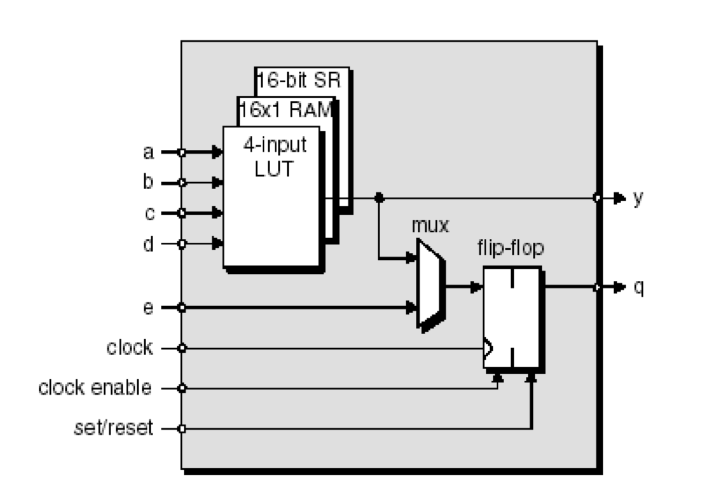
\includegraphics[width=0.5\textwidth,keepaspectratio=true]{./images/celda}
  \caption{Componentes de una celda lógica}
  \label{fig:esquema}
 \end{center}
\end{figure}

También se encuentran las \textit{Lookup Tables}, que son elementos lógicos que están compuestos de al menos un registro programable (flip\-flop) y alguna lógica de entrada, que usualmente está implementada como una lookup table de n entradas, donde n es 5 o menos. Estas LUTs son capaces de implementar cualquier función combinacional de sus entradas.

	\subsubsection{Bloques de Entrada y Salida de propósito general}

Las \textit{FPGAs} poseen pines TTL, CMOS, PCI, LVDS y muchos otros que les permiten hacer de interface y convertir muchas tecnologías diferentes. Las \textit{FPGAs} tienen bloques de I/O dedicados para clocks y resets globales.  

También incluyen PLL y esquemas para el manejo de clocks permitiendo múltiples dominios del mismo.Las \textit{FPGAs} actuales tienen impedancias de I/O configurables,  permiten el uso de resistencias internas terminales cuyos valores pueden ser configurados por el usuario.

\subsubsection{Multiplicadores}

Algunas funciones como los multiplicadores son muy lentos si se implementan mediante la conexión de un gran numero de bloques lógicos. Por eso muchas \textit{FPGAs} incorporan bloques \textit{multiplicadores} hardware. Estos bloques se encuentran muy cerca de los bloques de RAM embebidos. 

\begin{figure}[h!]
 \begin{center}
 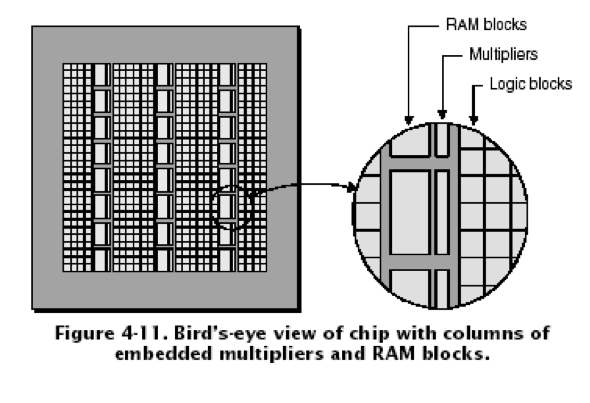
\includegraphics[width=0.5\textwidth,keepaspectratio=true]{./images/multram}
  \caption{Multiplicadores}
  \label{fig:esquema}
 \end{center}
\end{figure}

\subsubsection{Manejadores de Clock Digitales}

El \textit{clock manager} se usa para generar un número determinado de “daughter clocks". Es utilizado para remover el \textit{jitter}, como \textit{sintetizador de frecuencia} donde a partir de una frecuencia de referencia permite obtener un conjunto discreto de frecuencias, tratando de mantener en todos los casos las características de estabilidad de la frecuencia de referencia \cite{Etiqueta03}, también\textit{Phase shifting} algunos diseños requieren clocks que estén corridos en fase unos con respecto a otros.

\begin{figure}[h!]
 \begin{center}
 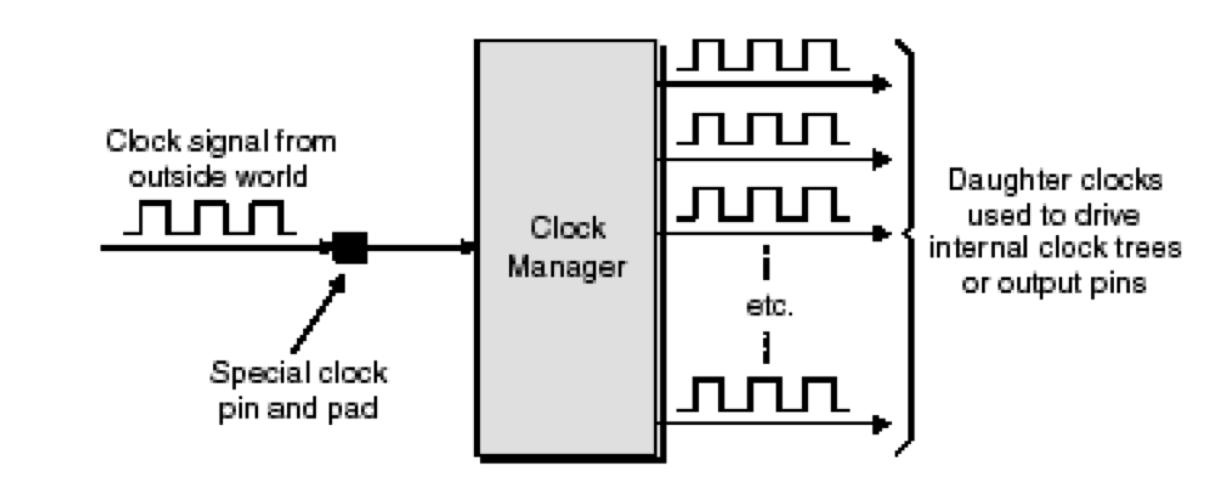
\includegraphics[width=0.5\textwidth,keepaspectratio=true]{./images/dougther}
  \caption{Clock Manager}
  \label{fig:esquema}
 \end{center}
\end{figure}

Se tiene  una estructura \textit{clock tree} por la que se distribuye la señal de clock principal que es ramificada para que alcance a todos los flip-flops. Esta estructura es así para asegurarse que todos los flip-flop estén lo mas cerca posible del clock y evitar el problema del \textit{skew}.

EL \textit{clock tree} es implementado usando canales separados de los de propósito general para interconectar los bloques.

\begin{figure}[h!]
 \begin{center}
 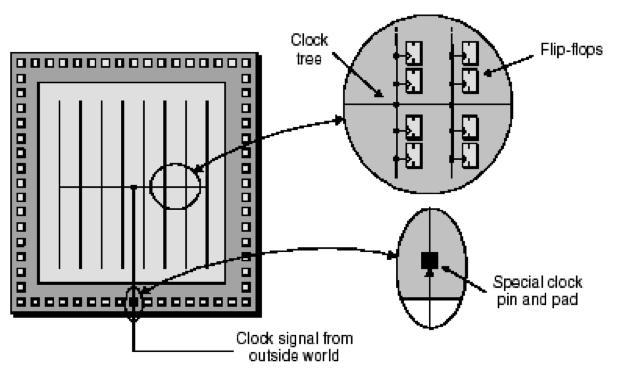
\includegraphics[width=0.5\textwidth,keepaspectratio=true]{./images/clocktree}
  \caption{Clock Tree}
  \label{fig:esquema}
 \end{center}
\end{figure}


\section{Microprocesadores Soft-Core reconfigurables}

 \subsection{Introducción}

EL avance en la en la tecnología de fabricación de VLSI (Very Large Scale Integratio) a medida que se agregaron más y más transistores,y en consecuencia más y más funciones fueron integradas en un mismo chip, por lo tanto también las capacidades en FPGAs. Grandes diseños de sistemas digitales que fueron sólo para ser implementado como ASICs, luego tuvieron la opción de ser ejecutados en FPGA.

El microprocesador, ya sea como un componente discreto o  como parte de otra lógica en el mismo chip, es una candidato  para ser  implementado en FPGA. Esto introdujo un mayor potencial para la exploración del espacio de diseño haciendo que la logica de computo especifica sea implemetada junto con un microprocesador estándar. \cite{Etiqueta05}

Dentro de los micro soft-core se encuetra un grupo apuntados principalmente a la re configuración de Hardware.
Tres de los más grandes proveedores de FPGA , Xilinx , Altera y Lattice , todos ofrecen sus propios núcleos de microprocesadores RISC de treinta y dos bits los dos mayores proveedores de dispositivos FPGA, Altera y Xilinx, proporcionan la Nios y Microblaze núcleos, respectivamente.

Existe un grupo de núcleos \textit{open source} que no están limitados por la tecnología, y son \textit{soft-cores}. Este grupo es desarrollado por lo general por aficionados en comunidades \textit{open source}, o en algunos casos, desarrollados por entidades comerciales antes de ser \textit{open source}.
 Para los desarrollos dirigidos a una re configuración de hardware la opción de microprocesadores \textit{Soft-Core} de treinta y dos bits se encuentra entre los que ofrecen los proveedores de FPGA y tambien disponible sin costo dentro de las comunidades \textit{open source}. Sin embargo , cuando se trata de ser capaz de desarrollar y vender un producto basado en estos \textit{cores}, hay consideraciones adicionales sobre la concesión de licencias de los diseños.

Las verdaderas ventajas de\textit{Soft-Core open source}, tienen que ver con la apertura del diseño, y la ausencia de restricciones sobre lo que se puede hacer con el \textit{core}. Con un diseño de código abierto existe la opción de personalizar la descripción RTL para implementar la optimización o la funcionalidad deseada. 

La portabilidad y la reutilización de producto final como su vigencia producto del acceso al diseño escrito en lenguaje de descripción de hardware tambien es una de las grandes ventajas de \textit{Soft-Core open source}.

		
		\subsubsection{ IP-Core}

El diseños de circuitos digitales se dividen normalmente en bloques funcionales, que se refiere como módulos, o \textit{cores}. Un \textit{core} estara formado por sub-bloques que ayudan a poner en práctica su funcionalidad. Los \textit{cores} pueden variar en tamaño hasta el tamaño total de un microprocesador. Un \textit{core} puede ocupar una FPGA entera al ser implementado, mientras que sólo se crea una instancia entre otros en una FPGA más grande o en un ASIC. Los \textit{núcleos} se describen generalmente utilizando un lenguaje de descripción de hardware (HDL) en un nivel de abstracción conocida como registro nivel de transferencia (RTL).

El proceso de tomar la descripción RTL de un diseño y convertirlo en un lista de primitivas o puertas lógicas y las conexiones entre ellos, dejando luego que la  implementación se realice en una tecnología de destino, se conoce como\textit{síntesis}. Analogamente a la compilación de software - que se tiene un programa en un lenguaje de alto nivel, como C, y  es convertido a codigo maquina. 

El resultado de la síntesis, conocida como una \textit{netlist}, está en un nivel de abstracción denominado nivel de la puerta.En pocas palabras, es esta lista de conexiones que se utiliza para su posterior procesamiento en una configuración para FPGA o en un diseño para ASIC.

Los cores pueden ser diseñados por una persona o entidad, los desarrolladores de \textit{cores} y licenciatarios varían en tamaño desde particulares a empresas de miles de millones de dólares. El producto, en este caso se conoce como un \textit{IP core  Intellectual Property Core} el diseño es la propiedad intelectual de los desarrolladores de terceros y la derecho a usarla recibe la licencia del cliente. La \textit{Intellectual Property IP} varia  de  acuerdo a las licencia.

		\paragraph{Tipos de IP-Cores}

\textit{IP} puede ser en una variedad de formas de acuerdo a la licencia. Las categorías con las que se clasifican los IP-Cores son:Hard-Cores, Firmes-core y soft-Cores.
		
			\subparagraph{Soft-Core}

Son los más flexibles y se presentan para \textit{IP} en forma netlist (lista de compuertas e interconexiones) o en forma de sintetizable RTL, lo que los hace tecnológicamente independientes.Los \textit{cores} sintetizable se entregan en un lenguaje de descripción de hardware como Verilog o VHDL. 
 Óptimos para diferentes aplicaciones, a costas de menor predictibilidad en la implementación y suelen tener un mayor costo y menor desempeño de procesamiento.

			\subparagraph{Firm-Core}

Los cores firmes están optimizados para ser implementados en una FPGA, arquitectura o dispositivo en particular. Esta optimización puede ser realizada por el fabricante o por un tercero. Utilizar este tipo de IP-Cores requiere disponer de cierto nivel de conocimiento de la arquitectura, ya que es posible rutear señales físicas y especificar la colocación de los elementos de diseño. Un ejemplo de cores firmes es el procesador MicroBlaze de Xilinx.\cite{Etiqueta04}

			\subparagraph{Hard-Core}

Están optimizados para una tecnología específica y no pueden ser modificados por el diseñador que los utiliza. Son manifestaciones físicas del diseño del core ya que tienen un layout predefinido incluido en la arquitectura. Son los mejores para aplicaciones plug\&play. Si bien son poco flexibles, portables y configurables, son muy predictibles (el timing es fijo) y fiables una vez implementados.
Si se trata de una forma menos abstraído forma , tal como un formato de un mensaje - diseño listo lista de conexiones o para la fabricación, que se conoce como
IP núcleo duro. \cite{Etiqueta04}

	
	%\subsection{Características de los micro Soft-Core}

\section{System on Chip}

 La capacidad de los ingenieros de diseño digital para hacer uso de transistores adicionales no ha seguido el ritmo de este incremento en la capacidad de fabricación \cite{Etiqueta05}. El tiempo para las necesidades del mercado de estos diseños cada vez más complejos permaneció fijo. 
Esto llevó a la aparición de la industria de IP core compuesta por empresas especializadas en el desarrollo de IP y concesión de licencias.

Esto permitio a los equipos de diseño montar un sistema formado por componentes básicos desarrollados por terceros para implementar el soporte para los protocolos de comunicación estándar, como Ethernet, IIC o SPI, mientras concentra sus esfuerzos de diseño en  lo que hace que su diseño único y particularmente valioso. Este es el caso de \textit{System on chip}.
En la mayoría de los casos un microprocesador es la parte mas complicada y esencial de un SoC, haciendo que el uso de IP pre-desarrollado una buena opción.

%Los métodos de la energía consciente de diseño y arquitecturas multi-core se han convertido , y es probable que siga siendo , una práctica estándar para los diseñadores SoC .


